%% chapter1_slides.tex
%% Beamer slides for Chapter 1: Background
%% "Convex Analysis and Monotone Operator Theory in Hilbert Spaces", 2nd ed.
%% Bauschke & Combettes -- CMS Books in Mathematics, Springer, 2017
%% Reader-friendly style: complete sentences, symbol explanations, worked examples
%% Compiled with: pdflatex -interaction=nonstopmode chapter1_slides.tex  (twice)
\documentclass[aspectratio=169,10pt]{beamer}

\usetheme{Madrid}
\usecolortheme{seahorse}
\usefonttheme{professionalfonts}

%% ── Packages ──────────────────────────────────────────────────────────────
\usepackage{amsmath,amssymb,amsfonts}
\usepackage{mathtools}
\usepackage{graphicx}
\usepackage{booktabs}
\usepackage{xcolor}
\usepackage{listings}

\graphicspath{{figures/}}

%% ── Python listing style ─────────────────────────────────────────────────
\lstdefinestyle{pycode}{
  language=Python,
  basicstyle=\ttfamily\scriptsize,
  numbers=left,
  numberstyle=\tiny\color{gray},
  frame=single,
  backgroundcolor=\color{gray!7},
  keywordstyle=\color{blue!70!black}\bfseries,
  commentstyle=\color{green!50!black}\itshape,
  stringstyle=\color{orange!80!black},
  showstringspaces=false,
  breaklines=true,
  tabsize=4,
  xleftmargin=1.5em,
  framexleftmargin=1.5em,
  aboveskip=4pt,
  belowskip=4pt,
}

%% ── Metadata ─────────────────────────────────────────────────────────────
\title[Convex Analysis \& MOT -- Ch.1]{Convex Analysis and Monotone Operator Theory in Hilbert Spaces}
\subtitle{Chapter 1: Background}
\author{Based on Bauschke \& Combettes}
\date{CMS Books in Mathematics, Springer, 2\textsuperscript{nd} ed., 2017}

\setbeamertemplate{footline}[frame number]
\setbeamertemplate{navigation symbols}{}

%% ── Helper macros ─────────────────────────────────────────────────────────
\DeclareMathOperator{\dom}{dom}
\DeclareMathOperator{\ran}{ran}
\DeclareMathOperator{\gra}{gra}
\DeclareMathOperator{\zer}{zer}
\DeclareMathOperator{\epi}{epi}
\DeclareMathOperator{\lev}{lev}
\DeclareMathOperator{\Fix}{Fix}
\DeclareMathOperator{\bdry}{bdry}
\DeclareMathOperator{\intr}{int}
\DeclareMathOperator{\cont}{cont}
\newcommand{\R}{\mathbb{R}}
\newcommand{\N}{\mathbb{N}}
\newcommand{\X}{\mathcal{X}}
\newcommand{\Y}{\mathcal{Y}}
\newcommand{\Z}{\mathcal{Z}}

%% ══════════════════════════════════════════════════════════════════════════
\begin{document}

%% ── Title frame ──────────────────────────────────────────────────────────
\begin{frame}
  \titlepage
\end{frame}

%% ── Outline ──────────────────────────────────────────────────────────────
\begin{frame}{Chapter Overview}
  \tableofcontents
\end{frame}

\AtBeginSection[]{\begin{frame}{Outline}\tableofcontents[currentsection]\end{frame}}

%% ══════════════════════════════════════════════════════════════════════════
\section{Why This Chapter Matters}
%% ══════════════════════════════════════════════════════════════════════════

\begin{frame}{Why This Chapter Matters}
  \begin{block}{The Purpose of Chapter 1}
    This chapter is the \textbf{vocabulary and toolbox} for the entire book.
    Nothing here is about convexity yet --- instead we fix the language of
    sets, operators, order, nets, extended real numbers, functions, topology,
    and metric spaces that every later chapter's proofs will use without
    re-explaining. Two books already in this repository (the
    \emph{Krasnosel'ski\u{i}--Mann Iterative Method} book and the
    \emph{$E$-values} book) build directly on the definitions given here.
  \end{block}
  \begin{alertblock}{How This Deck Is Organized}
    Every abstract definition is preceded by a one- or two-sentence plain
    English analogy, then the exact statement from the book, with every
    symbol explained. Two concrete running examples anchor the chapter:
    \begin{itemize}
      \item a specific \textbf{net} in $\R$ (indexed by the integers) that
        is unbounded overall yet still converges;
      \item a specific \textbf{lower semicontinuous function} on $\R$: the
        indicator function of a closed set versus the indicator function of
        a non-closed set.
    \end{itemize}
  \end{alertblock}
\end{frame}

%% ══════════════════════════════════════════════════════════════════════════
\section{Notation and Background You Need}
%% ══════════════════════════════════════════════════════════════════════════

\begin{frame}[allowframebreaks]{Notation and Background You Need}

  If you know basic real analysis and linear algebra but have never taken a
  topology or functional analysis course, read this frame first. Every term
  below is grounded in $\R$ or $\R^2$ before we ever state it abstractly.

  \begin{block}{Directed set (plain English: ``a notion of \emph{far enough
  along}'')}
    In $\N$ or $\R$, ``eventually'' means ``for all sufficiently large
    indices.'' A \textbf{directed set} $(A,\preccurlyeq)$ makes this precise
    for index sets that are not necessarily $\N$: any two indices $a,b$ have
    a common index $c$ that is ``further along'' than both ($a\preccurlyeq
    c$ and $b \preccurlyeq c$). This lets us say ``eventually'' even when the
    index set is, say, the open interval $\,]0,1[\,$.
  \end{block}

  \begin{block}{Net (plain English: ``a sequence whose index set need not be
  $\N$'')}
    A sequence $(x_n)_{n\in\N}$ assigns a point to every natural number. A
    \textbf{net} $(x_a)_{a\in A}$ does the same thing but for any directed
    set $A$. Every sequence is a net (take $A=\N$), but nets can be indexed
    by uncountable sets too, e.g., $A=\,]0,1[\,$. Nets are needed because in
    general topological spaces, sequences alone cannot always detect
    closures, continuity, or compactness --- nets can.
  \end{block}

  \begin{block}{Topological space (plain English: ``which sets count as
  `open{,}' abstracted away from any formula'')}
    In $\R^n$ you already know what an open set is (a union of open balls).
    A \textbf{topological space} simply declares, once and for all, a family
    of subsets to be called ``open'' (satisfying a few closure axioms),
    without needing a distance formula at all. Every metric space (like
    $\R^n$ with the usual distance) is an example, but the notion is more
    general: it is the minimal structure needed to talk about
    neighborhoods, closures, continuity, and convergence.

  \framebreak

  \end{block}

  \begin{block}{Hausdorff space (plain English: ``points can always be told
  apart'')}
    A topological space is \textbf{Hausdorff} if any two distinct points can
    be separated by disjoint open neighborhoods --- exactly as two distinct
    points in $\R^n$ can always be enclosed in two disjoint open balls.
    Every metric space is Hausdorff. This is assumed throughout the book so
    that limits are unique.
  \end{block}

  \begin{block}{Compactness (plain English: ``closed and bounded,''
  generalized)}
    In $\R^n$, compact means closed and bounded (Heine--Borel). In a general
    Hausdorff space, \textbf{compact} means: every open cover has a finite
    subcover. Equivalently (Fact~1.11 below), every net in the set has a
    subnet that converges to a point of the set.
  \end{block}

  \begin{block}{Extended real line $[-\infty,+\infty]$ (plain English:
  ``$\R$ plus two extra points at the ends'')}
    We adjoin two new symbols $-\infty$ and $+\infty$ to $\R$ so that every
    nonempty set of real numbers has a supremum and an infimum, even if it is
    unbounded. Arithmetic extends in the natural way, except that
    $+\infty+(-\infty)$, $0\cdot(+\infty)$, and $+\infty/+\infty$ are left
    undefined.

  \framebreak

  \end{block}

  \begin{block}{Lower semicontinuity (plain English: ``the function cannot
  suddenly jump \emph{down} in the limit, only up, and even an upward jump
  is fine as long as the value \emph{at} the point is the low one'')}
    Picture the graph of $f$ together with everything above it (the
    \textbf{epigraph}). $f$ is \textbf{lower semicontinuous (lsc)} at $x$ if,
    whenever points $x_a$ approach $x$, the function cannot sneak below its
    actual value $f(x)$ in the limit: $f(x) \le \varliminf f(x_a)$. A concrete
    picture: $f(x)=1$ for $x\ne 0$ and $f(0)=0$ is lsc (a downward dip is
    fine); but $f(x)=0$ for $x\ne0$ and $f(0)=1$ is \emph{not} lsc (an upward
    spike is not allowed, because nearby the value is lower than the limit
    would suggest). Equivalently: the epigraph is a \emph{closed} set.
  \end{block}

  \begin{block}{Sequential vs.\ topological notions (plain English:
  ``sequences are usually enough in $\R^n$, but not always in general
  spaces'')}
    Every definition above (closed, compact, continuous, lsc) has a
    ``sequential'' version obtained by using ordinary sequences $(x_n)_{n\in
    \N}$ instead of general nets. In metric spaces (in particular in
    $\R^n$) the sequential and topological versions always agree. In general
    topological spaces they can differ --- this is exactly why nets were
    introduced.

  \framebreak

  \end{block}

  \begin{block}{Cluster point (plain English: ``a point that the net/sequence
  keeps coming back near, even if it does not converge there'')}
    $x$ is a \textbf{cluster point} of $(x_a)_{a\in A}$ if the net is
    \emph{frequently} (not just eventually) in every neighborhood of $x$.
    Equivalently, some subnet converges to $x$. Example: the sequence
    $(-1)^n$ has cluster points $-1$ and $+1$, but does not converge.
  \end{block}

  \begin{block}{Metric space, Cauchy sequence, completeness (plain English:
  ``a space with a ruler, and a space with no missing limit points'')}
    A \textbf{metric space} $(\X,d)$ is a set equipped with a distance
    function $d$ satisfying the triangle inequality. A sequence is
    \textbf{Cauchy} if its terms eventually get arbitrarily close to each
    other (not necessarily to a known limit). The space is \textbf{complete}
    if every Cauchy sequence actually converges to a point of $\X$ --- i.e.,
    there are no ``holes'' where a limit ought to be. $\R^n$ with the usual
    distance is complete; $\mathbb{Q}$ is not (Cauchy sequences of rationals
    can converge to irrationals).
  \end{block}

\end{frame}

%% ══════════════════════════════════════════════════════════════════════════
\section{1.1 Sets in Vector Spaces}
%% ══════════════════════════════════════════════════════════════════════════

\begin{frame}{1.1 Sets in Vector Spaces}
  \textbf{Intuition.} Before defining operators and functions, the book fixes
  notation for the four possible ``line segments'' joining two points $x,y$
  in a vector space $\X$ --- open, closed, or half-open at either end, exactly
  as with real intervals $[x,y]$, $\,]x,y[\,$, etc.

  \begin{block}{The Four Types of Line Segments Between $x$ and $y$ in $\X$
  (1.3)}
    \[
      [x,y] = \{(1-\alpha)x + \alpha y \mid 0 \le \alpha \le 1\},
    \]
    \[
      \,]x,y[\, = \{(1-\alpha)x + \alpha y \mid 0 < \alpha < 1\}, \qquad
      [x,y[\, = \{(1-\alpha)x + \alpha y \mid 0 \le \alpha < 1\},
    \]
    and $\,]x,y] = [y,x[\,$.
    \begin{itemize}
      \item $\alpha \in [0,1]$ is a real \textbf{mixing weight}: $\alpha=0$
        gives $x$, $\alpha=1$ gives $y$, and intermediate $\alpha$ traces the
        straight segment between them.
      \item $[x,y]$ is the \textbf{closed} segment (both endpoints included);
        $\,]x,y[\,$ is the \textbf{open} segment (both endpoints excluded);
        $[x,y[\,$ and $\,]x,y]$ are \textbf{half-open}.
    \end{itemize}
  \end{block}

  \begin{alertblock}{Why This Matters Later}
    Convexity (Chapter 3 onward) is defined by requiring that $[x,y]\subset C$
    for every $x,y\in C$ --- so this exact notation for line segments is used
    on nearly every page of the rest of the book.
  \end{alertblock}
\end{frame}

%% ══════════════════════════════════════════════════════════════════════════
\section{1.2 Operators}
%% ══════════════════════════════════════════════════════════════════════════

\begin{frame}{1.2 Operators: Set-Valued Maps and Graphs}
  \textbf{Intuition.} An ordinary function sends each input to exactly one
  output. A \textbf{set-valued operator} sends each input to a whole
  \emph{set} of possible outputs --- think of a multi-valued ``menu'' rather
  than a single dish. This generality is essential for monotone operator
  theory (Chapters 20+), where objects like subdifferentials are naturally
  set-valued.

  \begin{block}{Operators and Set-Valued Operators}
    Let $\X,\Y,\Z$ be nonempty sets and let $2^\Y$ be the \textbf{power set}
    of $\Y$, i.e., the family of all subsets of $\Y$.
    \begin{itemize}
      \item $T:\X\to\Y$ means $T$ maps every point $x\in\X$ to a single point
        $Tx\in\Y$ (an ordinary \emph{operator}, also called a mapping).
      \item $A:\X\to2^\Y$ means $A$ maps every $x\in\X$ to a \emph{set}
        $Ax\subset\Y$ (a \textbf{set-valued operator}).
    \end{itemize}
  \end{block}

  \begin{block}{Graph of an Operator (1.4)}
    \[
      \gra A = \{(x,u)\in\X\times\Y \mid u\in Ax\}.
    \]
    The graph collects every input/output pair. If $C\subset\X$, then
    $A(C)=\bigcup_{x\in C}Ax$ is the image of $C$ under $A$.
  \end{block}
\end{frame}

\begin{frame}{1.2 Operators: Composition, Domain, Range, Inverse}
  \begin{block}{Composition (1.5)}
    Given $B:\Y\to2^\Z$, the composition of $A:\X\to2^\Y$ and $B$ is
    \[
      B\circ A:\X\to2^\Z: x\mapsto B(Ax)=\bigcup_{y\in Ax}By.
    \]
  \end{block}
  \begin{block}{Domain and Range (1.6)}
    \[
      \dom A = \{x\in\X \mid Ax\ne\varnothing\} \quad\text{and}\quad
      \ran A = A(\X).
    \]
    If $\X$ (resp.\ $\Y$) is a topological space, the closure of $\dom A$
    (resp.\ $\ran A$) is denoted $\overline{\dom}\,A$ (resp.\ $\overline{\ran}\,A$).
  \end{block}
  \begin{block}{Inverse (1.7)}
    \[
      \gra A^{-1} = \{(u,x)\in\Y\times\X \mid (x,u)\in\gra A\}.
    \]
    So $u\in Ax \Leftrightarrow x\in A^{-1}u$, and $\dom A^{-1}=\ran A$,
    $\ran A^{-1}=\dom A$.
  \end{block}
  \begin{block}{Zeros of an Operator (1.8)}
    If $\Y$ is a vector space, $\zer A = A^{-1}0 = \{x\in\X \mid 0\in Ax\}$.
    (Finding zeros of monotone operators is the central problem of
    Chapters 20--26.)
  \end{block}
\end{frame}

\begin{frame}{1.2 Operators: Single-Valued Operators, Selections, Special Classes}
  \begin{block}{At Most Single-Valued Operators, Selections (1.9)}
    Suppose $\dom A\ne\varnothing$. If $Ax=\{Tx\}$ is a singleton for every
    $x\in\dom A$, then $A$ is \textbf{at most single-valued} and identified
    with $T:\dom A\to\Y$. Conversely, any $T:D\to\Y$ (with $D\subset\X$
    nonempty) becomes the set-valued operator
    \[
      A:\X\to2^\Y: x\mapsto
      \begin{cases}
        \{Tx\}, & x\in D;\\
        \varnothing, & \text{otherwise.}
      \end{cases}
    \]
    A \textbf{selection} of $A:\X\to2^\Y$ is $T:\dom A\to\Y$ such that
    $Tx\in Ax$ for every $x\in\dom A$ --- a single-valued ``pick one'' rule
    consistent with $A$.
  \end{block}
  \begin{block}{Sums, Positive Homogeneity, Affine Maps (1.10)--(1.12)}
    If $\Y$ is a real vector space, $A,B:\X\to2^\Y$, $\lambda\in\R$, then
    $(A+\lambda B)x = Ax+\lambda Bx$. If $\X$ is a real vector space and
    $T:\X\to\Y$: $T$ is \textbf{positively homogeneous} if
    $T(\lambda x)=\lambda Tx$ for all $\lambda\in\R_{++}$ (strictly positive
    reals); $T$ is \textbf{affine} if
    $T(\lambda x+(1-\lambda)y)=\lambda Tx+(1-\lambda)Ty$ for all
    $x,y\in\X,\lambda\in\R$ -- equivalently, $x\mapsto Tx-T0$ is linear.
  \end{block}
  \begin{block}{Translation and Reversal}
    The \textbf{translation} of $A$ by $y\in\X$ is $\tau_yA: x\mapsto
    A(x-y)$; the \textbf{reversal} of $A$ is $A^\vee: x\mapsto A(-x)$.
  \end{block}
\end{frame}

\begin{frame}[fragile]{Python: Set-Valued Operators as Dictionaries of Sets}
  We represent a small set-valued operator $A:\{1,2,3\}\to 2^{\R}$ in Python
  as a dictionary mapping each input to a \texttt{set} of outputs, then
  compute its graph, domain, range, and inverse exactly as in (1.4)--(1.7).

  \begin{lstlisting}[style=pycode]
# A finite set-valued operator A: X -> 2^Y, X = {1,2,3}, Y subset of R
A = {1: {0.0, 1.0}, 2: {1.0}, 3: set()}  # A(3) = empty set: 3 not in dom A

def domain(A):
    return {x for x, vals in A.items() if len(vals) > 0}

def graph(A):
    return {(x, u) for x, vals in A.items() for u in vals}

def range_(A):
    return {u for vals in A.values() for u in vals}

def inverse(A):
    """Build A^{-1}: Y -> 2^X from gra(A^{-1}) = {(u,x) : (x,u) in gra(A)}."""
    Ainv = {}
    for (x, u) in graph(A):
        Ainv.setdefault(u, set()).add(x)
    return Ainv

print("dom A  =", domain(A))          # {1, 2}   (3 excluded: A(3) = empty)
print("gra A  =", graph(A))           # {(1,0.0), (1,1.0), (2,1.0)}
print("ran A  =", range_(A))          # {0.0, 1.0}
print("A^-1   =", inverse(A))         # {0.0: {1}, 1.0: {1, 2}}
print("zer A  =", {x for x in A if 0.0 in A[x]})   # {1}, since 0 in A(1)
  \end{lstlisting}
\end{frame}

%% ══════════════════════════════════════════════════════════════════════════
\section{1.3 Order}
%% ══════════════════════════════════════════════════════════════════════════

\begin{frame}{1.3 Order: Directed Sets and Partial Orders}
  \textbf{Intuition.} $\le$ on $\R$ is the model for all order relations:
  reflexive ($a\le a$), transitive, antisymmetric, and any two numbers are
  comparable. The book isolates exactly which of these properties are needed
  for different purposes (directedness for nets, antisymmetry for a genuine
  order).

  \begin{block}{Five Properties of a Binary Relation $\preccurlyeq$ on
  $A\times A$}
    \begin{enumerate}
      \item[\ding{172}] $(\forall a\in A)\; a\preccurlyeq a$ \hfill (reflexive)
      \item[\ding{173}] $a\preccurlyeq b,\,b\preccurlyeq c \Rightarrow
        a\preccurlyeq c$ \hfill (transitive)
      \item[\ding{174}] $(\forall a,b\in A)(\exists c\in A)\; a\preccurlyeq c
        \text{ and } b\preccurlyeq c$ \hfill (directed upward)
      \item[\ding{175}] $a\preccurlyeq b,\,b\preccurlyeq a \Rightarrow a=b$
        \hfill (antisymmetric)
      \item[\ding{176}] $(\forall a,b\in A)\; a\preccurlyeq b$ or
        $b\preccurlyeq a$ \hfill (total/comparable)
    \end{enumerate}
    We write $b\succcurlyeq a$ if $a\preccurlyeq b$.
  \end{block}

  \begin{block}{Directed Set, Partially Ordered Set (Poset), Strict Order (1.13)}
    If \ding{172}, \ding{173}, \ding{174} hold, $(A,\preccurlyeq)$ is a
    \textbf{directed set}. If \ding{172}, \ding{173}, \ding{175} hold,
    $(A,\preccurlyeq)$ is a \textbf{partially ordered set}; then the
    \textbf{strict order} is
    $a\prec b \Leftrightarrow [a\preccurlyeq b \text{ and } a\ne b]$.
    If, in addition, \ding{176} holds, $(A,\preccurlyeq)$ is \textbf{totally
    ordered}. Unless stated otherwise, $\R$ is totally ordered and directed
    by $\le$.
  \end{block}
\end{frame}

\begin{frame}{1.3 Order: Chains, Bounds, and Zorn's Lemma}
  \begin{block}{Chain, Upper/Lower Bound, Maximal Element}
    A totally ordered subset of a poset is called a \textbf{chain}. For
    $(A,\preccurlyeq)$ a poset and $B\subset A$: $a\in A$ is an
    \textbf{upper bound} of $B$ if $b\preccurlyeq a$ for every $b\in B$; a
    \textbf{lower bound} if $a\preccurlyeq b$ for every $b\in B$. $b\in B$ is
    the \textbf{least element} of $B$ if $b\preccurlyeq c$ for every $c\in
    B$. Finally, $a\in A$ is a \textbf{maximal element} of $A$ if
    $a\preccurlyeq c \Rightarrow c=a$ for every $c \in A$ (nothing in $A$ is
    strictly above $a$).
  \end{block}

  \begin{block}{Fact 1.1 (Zorn's Lemma)}
    Let $A$ be a partially ordered set such that every chain in $A$ has an
    upper bound. Then $A$ contains a maximal element.
  \end{block}

  \begin{alertblock}{Why It Is Called a ``Lemma'' but Cannot Be Proved}
    Zorn's Lemma is logically \emph{equivalent} to the Axiom of Choice; it is
    taken as an axiom of set theory, not derived from more elementary facts.
    It will be used later in the book (e.g., to extend linear functionals,
    or to find maximal monotone extensions) whenever an explicit
    construction of a maximal object is not available.
  \end{alertblock}

  \begin{exampleblock}{Concrete Instance}
    Figure~1 (next section) shows a small finite poset with a chain
    $a\prec b\prec d\prec g$; the element $g$ is both an upper bound of that
    chain and a maximal element of the whole poset --- exactly the
    conclusion Zorn's Lemma guarantees in general (infinite) posets.
  \end{exampleblock}
\end{frame}

\begin{frame}{Figure: A Poset, a Chain, and a Maximal Element}
  \begin{center}
    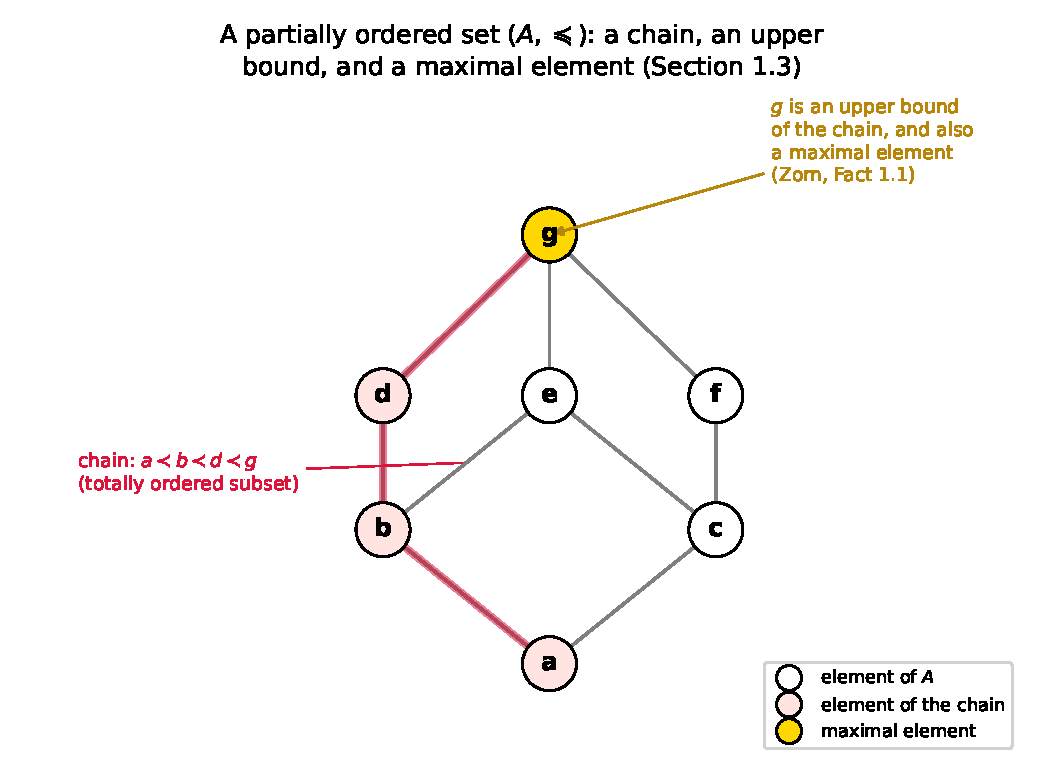
\includegraphics[width=0.62\linewidth]{fig_order_zorn.pdf}
  \end{center}
  \small The finite poset $(A,\preccurlyeq)$ shown here is ordered ``upward''
  along the edges (e.g., $a\prec b$, $b\prec d$, $d\prec g$). The highlighted
  chain $a\prec b\prec d\prec g$ is totally ordered. The element $g$ sits
  above every element of the chain (an upper bound) and above every other
  element of $A$ that is comparable to it, so $g$ is also a maximal element
  --- consistent with Fact~1.1.
\end{frame}

%% ══════════════════════════════════════════════════════════════════════════
\section{1.4 Nets}
%% ══════════════════════════════════════════════════════════════════════════

\begin{frame}{1.4 Nets: Definition, Eventually, Frequently}
  \textbf{Intuition.} A net generalizes a sequence to arbitrary directed
  index sets. ``Eventually in $\Y$'' means ``from some index onward, always
  in $\Y$'' (like tail behavior of a sequence); ``frequently in $\Y$'' means
  ``no matter how far you go, you can still find a later index back in
  $\Y$'' (like a subsequence keeps returning).

  \begin{block}{Net (Generalized Sequence)}
    Let $(A,\preccurlyeq)$ be a directed set and $\X$ a nonempty set. A
    \textbf{net} in $\X$ indexed by $A$ is an operator from $A$ to $\X$,
    denoted $(x_a)_{a\in A}$. Since $(\N,\le)$ is directed, every sequence is
    a net; but there are nets that are not sequences, e.g.,
    $(a)_{a\in\,]0,1[}$.
  \end{block}

  \begin{block}{Eventually / Frequently in $\Y\subset\X$ (1.14)--(1.15)}
    \[
      (x_a)_{a\in A} \text{ is \emph{eventually} in } \Y \;:\Leftrightarrow\;
      (\exists c\in A)(\forall a\in A)\; a\succcurlyeq c \Rightarrow x_a\in\Y,
    \]
    \[
      (x_a)_{a\in A} \text{ is \emph{frequently} in } \Y \;:\Leftrightarrow\;
      (\forall c\in A)(\exists a\in A)\; a\succcurlyeq c \text{ and } x_a\in\Y.
    \]
    ``Eventually'' says the net enters $\Y$ and stays; ``frequently'' says it
    keeps coming back to $\Y$, though it may also leave again.
  \end{block}
\end{frame}

\begin{frame}{1.4 Nets: Subnets and a Cautionary Remark}
  \begin{block}{Subnet (1.16)--(1.17)}
    A net $(y_b)_{b\in B}$ is a \textbf{subnet} of $(x_a)_{a\in A}$ via
    $k:B\to A$ if $y_b = x_{k(b)}$ for every $b\in B$, and
    \[
      (\forall a\in A)(\exists d\in B)(\forall b\in B)\; b\succcurlyeq d
      \Rightarrow k(b)\succcurlyeq a.
    \]
    In words: $k$ eventually outruns any given index $a$ of the original
    net. When $A=B=\N$ and $k$ is strictly increasing, a subnet is precisely
    a \textbf{subsequence} --- but in general subnets are a strictly broader
    notion.
  \end{block}

  \begin{alertblock}{Remark 1.2: A Subnet Need Not Be a Subsequence}
    Let $B\subset\R$ be nonempty and unbounded above, and let $k:B\to\N$
    satisfy $k(b)\to+\infty$ as $b\to+\infty$. Then $(x_{k(b)})_{b\in B}$ is
    a subnet of $(x_n)_{n\in\N}$. If $B$ is uncountable, it is not even a
    subsequence (a subsequence's index set must be countable and embed
    order-preservingly into $\N$). Likewise, if $B=\N$ but $k$ is not
    strictly increasing (e.g., $k(b)=b(2+(-1)^b)$), the result is a subnet
    but not a subsequence.
  \end{alertblock}

  \begin{exampleblock}{Running Example: A Net That Is Unbounded Yet Convergent}
    Let $A=\mathbb Z$, directed by $\le$ (so ``eventually'' means ``for all
    sufficiently large integers,'' since $\Z$ has no largest element in the
    other direction --- directedness only requires common upper bounds).
    Define $x_a = a$ for $a\le0$ and $x_a=1/a$ for $a>0$ (Exercise 1.4). We
    will show on the next slide that $(x_a)_{a\in A}$ converges to $0$ even
    though, as a whole set of values, it is unbounded below.
  \end{exampleblock}
\end{frame}

\begin{frame}{Running Example: Net Convergence Only Depends on the Tail}
  \begin{columns}[T]
    \column{0.52\linewidth}
      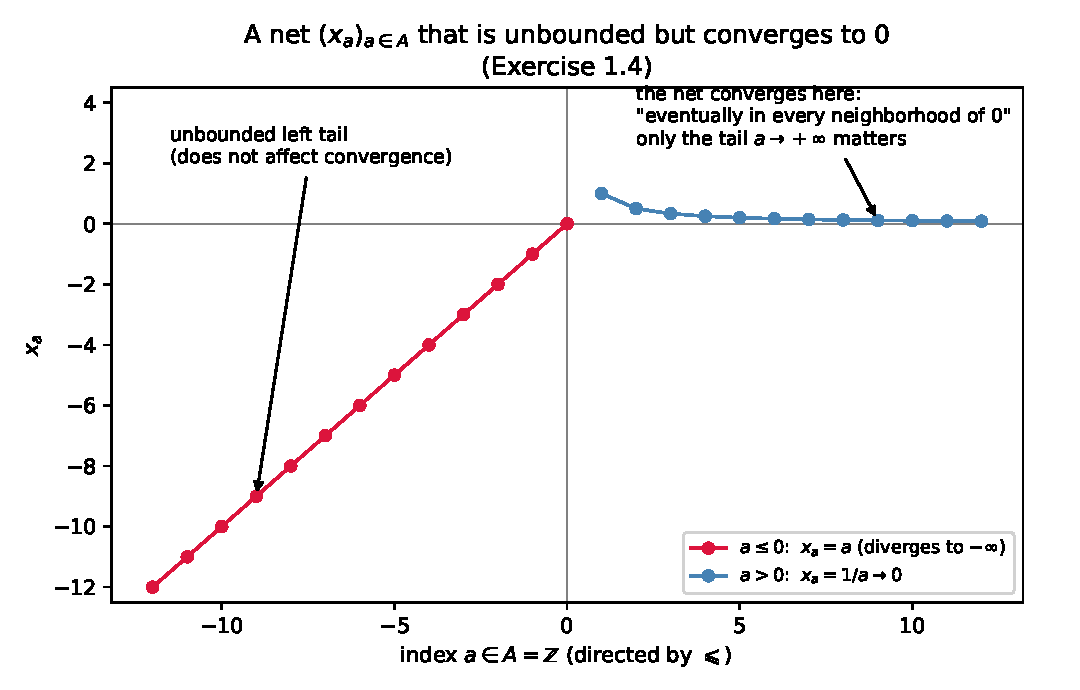
\includegraphics[width=\linewidth]{fig_net_convergence.pdf}
    \column{0.46\linewidth}
      \begin{block}{Why This Net Converges to $0$}
        \textbf{Step 1.} Fix any neighborhood $V=\,]-\varepsilon,\varepsilon[\,$
        of $0$, $\varepsilon>0$.

        \smallskip
        \textbf{Step 2.} Choose $c\in A=\Z$ with $c>1/\varepsilon$ and
        $c>0$.

        \smallskip
        \textbf{Step 3.} For every $a\succcurlyeq c$ (i.e., every integer
        $a\ge c$), we have $a>0$, so $x_a=1/a\le 1/c<\varepsilon$; hence
        $x_a\in V$.

        \smallskip
        \textbf{Conclusion.} $(x_a)_{a\in A}$ is eventually in every
        neighborhood of $0$, so $x_a\to0$ by (1.26) below --- even though
        $\{x_a : a\in A\}$ is unbounded (because $x_a=a\to-\infty$ for
        $a\le0$). \textbf{Convergence of a net is purely a tail
        property.}
      \end{block}
  \end{columns}
\end{frame}

\begin{frame}[fragile]{Python: Verifying Net Convergence Numerically}
  We check, for the running example, that the tail of the net (as $a\to
  +\infty$) enters and stays inside shrinking neighborhoods of $0$, exactly
  as predicted by the eventual/frequently definitions (1.14)--(1.15).

  \begin{lstlisting}[style=pycode]
def x(a):
    """The net from Exercise 1.4: x_a = a if a <= 0, else 1/a."""
    return float(a) if a <= 0 else 1.0 / a

def eventually_in_ball(radius, search_range=10_000):
    """Smallest index c such that x_a in (-radius, radius) for all a >= c."""
    for c in range(1, search_range):
        if all(abs(x(a)) < radius for a in range(c, c + 50)):
            return c
    return None

for eps in [0.1, 0.01, 0.001]:
    c = eventually_in_ball(eps)
    print(f"eps={eps:<6} -> eventually in (-eps,eps) from index c={c}, "
          f"x_c={x(c):.5f}")
# eps=0.1    -> eventually in (-eps,eps) from index c=11, x_c=0.09091
# eps=0.01   -> eventually in (-eps,eps) from index c=101, x_c=0.00990
# eps=0.001  -> eventually in (-eps,eps) from index c=1001, x_c=0.00100
# Meanwhile x(-10000) = -10000: the net is unbounded, yet still converges.
print("x(-10000) =", x(-10000), "  (net values are unbounded below)")
  \end{lstlisting}
\end{frame}

%% ══════════════════════════════════════════════════════════════════════════
\section{1.5 The Extended Real Line}
%% ══════════════════════════════════════════════════════════════════════════

\begin{frame}{1.5 The Extended Real Line: Notation}
  \textbf{Intuition.} Adjoining $\pm\infty$ to $\R$ guarantees every set of
  reals has a supremum and infimum, which is indispensable once we allow
  functions to take the value $+\infty$ (as convex analysis routinely does,
  e.g., for indicator functions).

  \begin{block}{The Extended Real Line}
    $[-\infty,+\infty] = \R\cup\{-\infty\}\cup\{+\infty\}$, with the order
    extended by $-\infty<\xi<+\infty$ for every $\xi\in\R$. Arithmetic
    extends naturally, \emph{except} that $+\infty+(-\infty)$,
    $0\cdot(+\infty)$, and $+\infty/+\infty$ remain \textbf{undefined}
    unless stated otherwise.
  \end{block}

  \begin{block}{Remark 1.3: Sign and Orthant Terminology}
    For extended reals: \emph{positive} means $\ge0$, \emph{strictly
    positive} means $>0$ (similarly negative/strictly negative with $\le0,
    <0$). $\R_+=[0,+\infty[\,$, $\R_{++}=\,]0,+\infty[\,$. For a strictly
    positive integer $N$, the \textbf{positive orthant} is
    $\R^N_+=[0,+\infty[^{\,N}$ and the \textbf{strictly positive orthant} is
    $\R^N_{++}=\,]0,+\infty[^{\,N}$ (with $\R^N_-,\R^N_{--}$ defined
    similarly).
  \end{block}

  \begin{block}{Increasing / Decreasing Functions}
    $f:D\to[-\infty,+\infty]$ (with $D\subset\R$) is \textbf{increasing} if
    $\xi<\eta \Rightarrow f(\xi)\le f(\eta)$ (\textbf{strictly increasing} if
    $f(\xi)<f(\eta)$). Applying this to $-f$ gives \emph{decreasing} and
    \emph{strictly decreasing}.
  \end{block}
\end{frame}

\begin{frame}{1.5 Infimum, Supremum, and Limits of a Net}
  \begin{block}{Infimum and Supremum}
    Let $S\subset[-\infty,+\infty]$. The \textbf{infimum} $\inf S$ is the
    unique greatest lower bound of $S$ (written $\min S$ when $\inf S\in
    S$); the \textbf{supremum} $\sup S = -\inf\{-\alpha \mid \alpha\in S\}$
    (written $\max S$ when $\sup S\in S$). Every set $S$ has both an
    infimum and a supremum in $[-\infty,+\infty]$; by convention
    $\inf\varnothing=+\infty$ and $\sup\varnothing=-\infty$.
  \end{block}

  \begin{block}{Limit Inferior and Limit Superior of a Net (1.18)--(1.19)}
    For a net $(\xi_a)_{a\in A}$ in $[-\infty,+\infty]$,
    \[
      \varliminf_a \xi_a = \sup_{a\in A}\;\inf_{\substack{b\in A\\ a\preccurlyeq b}} \xi_b,
      \qquad
      \varlimsup_a \xi_a = \inf_{a\in A}\;\sup_{\substack{b\in A\\ a\preccurlyeq b}} \xi_b.
    \]
    The inner $\inf$ (resp.\ $\sup$) over the ``tail'' $\{b\succcurlyeq a\}$
    is nondecreasing (resp.\ nonincreasing) as $a$ grows, so the outer
    $\sup$ (resp.\ $\inf$) captures the eventual worst-case lower (resp.\
    upper) behavior. It is always true that
    $\varliminf_a\xi_a \le \varlimsup_a\xi_a$.
  \end{block}

  \begin{exampleblock}{Running Example}
    For our net $x_a=a\;(a\le0)$, $x_a=1/a\;(a>0)$: since the net converges
    to $0$ (shown two slides ago), $\varliminf x_a=\varlimsup x_a=0$, even
    though $\inf\{x_a\}=-\infty$ over the whole index set. Limit inferior /
    superior only see the eventual tail, exactly like ordinary limits.
  \end{exampleblock}
\end{frame}

\begin{frame}[fragile]{Python: Computing $\varliminf$ and $\varlimsup$ of a Net}
  This code computes the tail infima/suprema in (1.18)--(1.19) directly from
  the definitions, for both our running net and the classical sequence
  $(-1)^n$, whose liminf/limsup do \emph{not} coincide.

  \begin{lstlisting}[style=pycode]
import math

def tail_inf_sup(values, a):
    """inf and sup of {x_b : b >= a} for a finite window of a sequence."""
    tail = values[a:]
    return (min(tail) if tail else math.inf,
            max(tail) if tail else -math.inf)

def liminf_limsup(values):
    """Approximate (1.18)-(1.19) using a long but finite index window."""
    n = len(values)
    tail_infs = [tail_inf_sup(values, a)[0] for a in range(n)]
    tail_sups = [tail_inf_sup(values, a)[1] for a in range(n)]
    return max(tail_infs), min(tail_sups)   # sup_a inf_{b>=a}, inf_a sup_{b>=a}

# Running example net restricted to a >= 1 (finite window a = 1..N)
N = 2000
net_vals = [1.0 / a for a in range(1, N + 1)]
li, ls = liminf_limsup(net_vals)
print(f"running example: liminf = {li:.4f}, limsup = {ls:.4f}  (both -> 0)")

# Classical example with NO limit: (-1)^n
osc_vals = [(-1) ** n for n in range(N)]
li2, ls2 = liminf_limsup(osc_vals)
print(f"(-1)^n:          liminf = {li2}, limsup = {ls2}  (differ: no limit)")
  \end{lstlisting}
\end{frame}

%% ══════════════════════════════════════════════════════════════════════════
\section{1.6 Functions}
%% ══════════════════════════════════════════════════════════════════════════

\begin{frame}{1.6 Functions: Domain, Graph, Epigraph, Level Sets}
  \textbf{Intuition.} A function $f$ into the extended reals may take the
  value $+\infty$; the set where $f$ is finite is its (effective) domain.
  The \textbf{epigraph} --- everything on or above the graph --- turns
  analytic properties of $f$ (like lower semicontinuity, or later,
  convexity) into geometric properties of a set.

  \begin{block}{Definition 1.4: Domain, Graph, Epigraph, Level Sets}
    Let $f:\X\to[-\infty,+\infty]$.
    \[
      \dom f = \{x\in\X \mid f(x)<+\infty\}, \qquad
      \gra f = \{(x,\xi)\in\X\times\R \mid f(x)=\xi\},
    \]
    \[
      \epi f = \{(x,\xi)\in\X\times\R \mid f(x)\le\xi\}, \qquad
      \lev_{\le\xi} f = \{x\in\X \mid f(x)\le\xi\},
    \]
    \[
      \lev_{<\xi} f = \{x\in\X \mid f(x)<\xi\}.
    \]
    $f$ is \textbf{proper} if $-\infty\notin f(\X)$ and $\dom f\ne
    \varnothing$ (it never takes the value $-\infty$, and it is not
    identically $+\infty$).
  \end{block}

  \begin{alertblock}{Remark 1.5}
    $\dom f$ is sometimes called the \emph{effective domain}, since $f$ as
    an operator is really defined on all of $\X$ (with value possibly
    $+\infty$). If $f,g:\X\to[-\infty,+\infty]$, their sum uses the
    convention $+\infty+(-\infty)=+\infty$, so
    $\dom(f+g)=\dom f\cap\dom g$.
  \end{alertblock}
\end{frame}

\begin{frame}{1.6 Lemma 1.6: Epigraphs of Suprema and Minima}
  \textbf{Intuition.} Taking the pointwise supremum of a family of functions
  corresponds \emph{exactly} to intersecting their epigraphs; taking the
  minimum of finitely many functions corresponds to taking the union of
  their epigraphs.

  \begin{block}{Lemma 1.6}
    Let $(f_i)_{i\in I}$ be functions from $\X$ to $[-\infty,+\infty]$. Then
    \begin{enumerate}
      \item[(i)] $\epi(\sup_{i\in I} f_i) = \bigcap_{i\in I}\epi f_i$.
      \item[(ii)] If $I$ is finite, $\epi(\min_{i\in I} f_i) =
        \bigcup_{i\in I}\epi f_i$.
    \end{enumerate}
  \end{block}

  \begin{exampleblock}{Proof of (i), Step by Step}
    Take $(x,\xi)\in\X\times\R$.
    \begin{itemize}
      \item \textbf{Step 1.} $(x,\xi)\in\epi(\sup_i f_i)
        \Leftrightarrow \sup_i f_i(x)\le\xi$.
      \item \textbf{Step 2.} $\sup_i f_i(x)\le\xi \Leftrightarrow
        (\forall i\in I)\; f_i(x)\le\xi$ (a supremum is $\le\xi$ exactly
        when every term is $\le\xi$).
      \item \textbf{Step 3.} $(\forall i\in I)\, f_i(x)\le\xi
        \Leftrightarrow (\forall i\in I)\,(x,\xi)\in\epi f_i
        \Leftrightarrow (x,\xi)\in\bigcap_i \epi f_i$.
    \end{itemize}
    Part (ii) follows the same three steps with $\min$/``some $i$''/union in
    place of $\sup$/``every $i$''/intersection.
  \end{exampleblock}
\end{frame}

\begin{frame}{1.6 Infimum/Supremum over a Subset, Minimizing Sequences}
  \begin{block}{Definition 1.7: Infimum/Supremum of $f$ over $C\subset\X$}
    $\inf f(C) := \inf_{x\in C} f(x)$. $f$ \textbf{achieves its infimum} over
    $C$ if there is $y\in C$ with $f(y)=\inf f(C)$; then we write
    $f(y)=\min f(C)$. Similarly for $\sup f(C)$ and $\max f(C)$.
  \end{block}
  \begin{block}{Definition 1.8: Minimizing Sequence}
    $(x_n)_{n\in\N}$ in $\dom f$ is a \textbf{minimizing sequence} of $f$ if
    $f(x_n)\to \inf f(\X)$: its function values approach the global infimum,
    even if the points $x_n$ themselves do not converge to any single
    minimizer (or even if no minimizer exists at all).
  \end{block}
  \begin{block}{Translation and Reversal of a Function}
    If $\X$ is a real vector space and $f:\X\to[-\infty,+\infty]$: the
    \textbf{translation} of $f$ by $y\in\X$ is $\tau_y f: x\mapsto f(x-y)$;
    the \textbf{reversal} is $f^\vee: x\mapsto f(-x)$.
  \end{block}
  \begin{alertblock}{Why Minimizing Sequences Matter}
    Much of optimization theory (Chapters 11+) is precisely about showing
    that a minimizing sequence converges (in some sense) to an actual
    minimizer. Weierstrass's theorem (Theorem 1.29, coming up in Section
    1.10) is the prototypical result guaranteeing that a minimizer exists.
  \end{alertblock}
\end{frame}

\begin{frame}[fragile]{Python: Epigraphs and Level Sets, Numerically}
  We plot/sample the epigraph and lower level sets of a concrete function
  $f(x)=x^2$ restricted to $x\in[-2,2]$, and verify Lemma~1.6(ii) numerically
  for $\min(f,g)$ with $g(x)=(x-1)^2$.

  \begin{lstlisting}[style=pycode]
import numpy as np

def f(x): return x**2
def g(x): return (x - 1)**2

xs = np.linspace(-2, 2, 9)
xi = 1.0  # test height for the epigraph / level-set membership

# Lower level set lev_{<=1} f = {x : f(x) <= 1}
lev_f = [x for x in xs if f(x) <= xi]
print("lev_{<=1} f =", lev_f)   # should be x in [-1, 1] (sampled grid)

# Verify epi(min(f,g)) == epi(f) union epi(g)  pointwise, at height xi
for x in xs:
    lhs = min(f(x), g(x)) <= xi                     # (x, xi) in epi(min(f,g))?
    rhs = (f(x) <= xi) or (g(x) <= xi)               # (x, xi) in epi f U epi g?
    assert lhs == rhs, (x, lhs, rhs)
print("Lemma 1.6(ii) verified pointwise: epi(min(f,g)) == epi(f) U epi(g)")
  \end{lstlisting}
\end{frame}

%% ══════════════════════════════════════════════════════════════════════════
\section{1.7 Topological Spaces}
%% ══════════════════════════════════════════════════════════════════════════

\begin{frame}{1.7 Topology, Base, Interior, Closure, Boundary}
  \textbf{Intuition.} A topology is the minimal bookkeeping needed to say
  which sets are ``open'' without reference to a distance formula; every
  metric space (like $\R^n$) gives rise to one, but the notion applies far
  more generally.

  \begin{block}{Topology, Topological Space, Open/Closed, Neighborhood}
    A \textbf{topology} $\mathsf T$ on $\X$ is a family of subsets of $\X$
    containing $\X$, $\varnothing$, all arbitrary unions, and all finite
    intersections of its members. $(\X,\mathsf T)$ is a \textbf{topological
    space}. Members of $\mathsf T$ are \textbf{open}; their complements are
    \textbf{closed}. A \textbf{neighborhood} of $x$ is a set $V\supset U$ for
    some open $U\ni x$; $\mathcal V(x)$ denotes the family of all
    neighborhoods of $x$.
  \end{block}

  \begin{block}{Base, Interior, Closure, Boundary, Dense, Product Topology (1.25)}
    A subfamily $\mathsf B\subset\mathsf T$ is a \textbf{base} of $\mathsf T$
    if every $V\in\mathcal V(x)$ contains some $B\in\mathsf B$ with $x\in B$.
    For $C\subset\X$: $\intr C$ is the largest open set inside $C$;
    $\overline C$ is the smallest closed set containing $C$; $C$ is
    \textbf{dense} if $\overline C=\X$; the \textbf{boundary} is $\bdry
    C=\overline C\smallsetminus\intr C$. The \textbf{product topology} on
    $\X_1\times\X_2$ has base $\mathsf B=\{B_1\times B_2 \mid B_1\in
    \mathsf B_1, B_2\in\mathsf B_2\}$.
  \end{block}
\end{frame}

\begin{frame}{1.7 Hausdorff Spaces, Compactness, Convergence of Nets}
  \begin{block}{Hausdorff Space, Compact Set}
    $\X$ is \textbf{Hausdorff} if any two distinct points $x_1\ne x_2$ admit
    disjoint neighborhoods $V_1\in\mathcal V(x_1)$, $V_2\in\mathcal V(x_2)$.
    A subset $C$ of a Hausdorff space is \textbf{compact} if every open
    cover of $C$ has a finite subcover.
  \end{block}
  \begin{block}{Convergence of a Net (1.26)}
    A net $(x_a)_{a\in A}$ \textbf{converges} to $x\in\X$ (written $x_a\to
    x$ or $\lim x_a=x$; the limit is necessarily unique in a Hausdorff
    space) if it lies eventually in every neighborhood of $x$:
    \[
      (\forall V\in\mathcal V(x))(\exists b\in A)(\forall a\in A)\;
      a\succcurlyeq b \Rightarrow x_a\in V.
    \]
  \end{block}
  \begin{exampleblock}{Instantiating (1.26) with the Running Example}
    For $A=\Z$, $x_a=a$ $(a\le0)$, $x_a=1/a$ $(a>0)$: we already verified
    (two slides ago) exactly this definition with $x=0$ and $V=\,]-\varepsilon,
    \varepsilon[\,$, obtaining $x_a\to0$.
  \end{exampleblock}
\end{frame}

\begin{frame}{1.7 Cluster Points and Their Characterization via Subnets}
  \begin{block}{Fact 1.9}
    If $x_a\to x$ in a Hausdorff space and $(x_{k(b)})_{b\in B}$ is a subnet
    of $(x_a)_{a\in A}$, then $x_{k(b)}\to x$: subnets of convergent nets
    converge to the same limit.
  \end{block}
  \begin{block}{Cluster Point (1.27)}
    $x\in\X$ is a \textbf{cluster point} (or accumulation point) of
    $(x_a)_{a\in A}$ if the net lies \emph{frequently} in every neighborhood
    of $x$:
    \[
      (\forall V\in\mathcal V(x))(\forall b\in A)(\exists a\in A)\;
      a\succcurlyeq b \text{ and } x_a\in V.
    \]
    Equivalently, $x$ is a cluster point iff $(x_a)_{a\in A}$ possesses a
    subnet converging to $x$. If a \emph{sequence} $(x_n)_{n\in\N}$ has a
    subsequence converging to $x$, then $x$ is called a \textbf{sequential
    cluster point} of $(x_n)_{n\in\N}$.
  \end{block}
  \begin{alertblock}{Topological Notions via Nets}
    The next lemma shows nets can \emph{characterize} closures purely in
    terms of convergence -- a template used repeatedly in this book instead
    of reasoning about open covers directly.
  \end{alertblock}
\end{frame}

\begin{frame}{1.7 Lemma 1.10: Closures via Nets}
  \begin{block}{Lemma 1.10}
    Let $C$ be a subset of a Hausdorff space $\X$ and $x\in\X$. Then $x\in
    \overline C$ if and only if there exists a net in $C$ that converges to
    $x$.
  \end{block}
  \begin{exampleblock}{Proof, Step by Step}
    \textbf{($\Rightarrow$) Step 1.} Suppose $x\in\overline C$. Direct
    $A=\mathcal V(x)$ by $a\preccurlyeq b \Leftrightarrow a\supset b$ (bigger
    neighborhoods come ``first''). \textbf{Step 2.} Since $x\in\overline
    C$, every $a\in A$ satisfies $C\cap a\ne\varnothing$; pick $x_a\in
    C\cap a$. \textbf{Step 3.} The net $(x_a)_{a\in A}$ lies in $C$ and
    converges to $x$ by construction (given $V\in\mathcal V(x)$, take
    $b=V$: for $a\preccurlyeq b$, $x_a \in a \subset b=V$).

    \smallskip
    \textbf{($\Leftarrow$) Step 1.} Suppose a net $(x_a)_{a\in A}$ in $C$
    converges to $x$. \textbf{Step 2.} Fix $V\in\mathcal V(x)$; by
    convergence, $(x_a)$ is eventually in $V$, so some $x_a\in C\cap V$,
    giving $C\cap V\ne\varnothing$. \textbf{Step 3.} Since this holds for
    every $V\in\mathcal V(x)$, we conclude $x\in\overline C$.
  \end{exampleblock}
  \begin{block}{Consequence}
    $C$ is closed iff the limit of every convergent net in $C$ lies in $C$.
    $C$ is open iff, for every $x\in C$, every net converging to $x$ is
    eventually in $C$.
  \end{block}
\end{frame}

\begin{frame}{1.7 Fact 1.11 and Compactness via Nets}
  \begin{block}{Fact 1.11: Equivalent Characterizations of Compactness}
    Let $C$ be a subset of a Hausdorff space $\X$. The following are
    equivalent:
    \begin{enumerate}
      \item[(i)] $C$ is compact.
      \item[(ii)] $C\cap\bigcap_{j\in J}C_j\ne\varnothing$ for every family
        $(C_j)_{j\in J}$ of closed sets such that every finite
        subintersection with $C$ is nonempty.
      \item[(iii)] Every net in $C$ has a cluster point in $C$.
      \item[(iv)] Every net in $C$ has a subnet converging to a point in $C$.
    \end{enumerate}
  \end{block}
  \begin{block}{Lemma 1.12 and Remark 1.13}
    A compact subset $C$ of a Hausdorff space is \textbf{closed}, and every
    closed subset of $C$ is compact (proof: extract a convergent subnet via
    Fact~1.11, use uniqueness of limits in a Hausdorff space). \textbf{Caution
    (Remark 1.13):} a compact set's sequences always have a convergent
    \emph{subnet}, but in general topological spaces they need not have a
    convergent \emph{subsequence}.
  \end{block}
  \begin{block}{Lemma 1.14: Unique Cluster Point Implies Convergence}
    If $(x_a)_{a\in A}$ lies in a compact $C$ and has a \emph{unique}
    cluster point $x$, then $x_a\to x$ (proved by contradiction using
    Lemma~1.12: if not, a subnet stays away from $x$ inside the compact set
    $C\smallsetminus V$ and produces a second cluster point).
  \end{block}
\end{frame}

%% ══════════════════════════════════════════════════════════════════════════
\section{1.8 Two-Point Compactification of the Real Line}
%% ══════════════════════════════════════════════════════════════════════════

\begin{frame}{1.8 Two-Point Compactification of the Real Line}
  \textbf{Intuition.} $\R$ itself is not compact (it is unbounded), but
  adding the two ``endpoints'' $\pm\infty$ and giving them suitable
  neighborhoods (rays $[-\infty,\xi[\,$ and $\,]\xi,+\infty]$) turns
  $[-\infty,+\infty]$ into a compact space -- exactly like adding two caps to
  a line to make a circle-like compact object.

  \begin{block}{The Topology of $[-\infty,+\infty]$}
    $\R$ carries its usual topology (base: open intervals), making it
    Hausdorff but not compact. $[-\infty,+\infty]$ carries the topology with
    base the open real intervals together with $[-\infty,\xi[\,$ and
    $\,]\xi,+\infty]$ for $\xi\in\R$; this makes $[-\infty,+\infty]$ a
    \textbf{compact} Hausdorff space.
  \end{block}

  \begin{block}{Fact 1.15: Nets in $[-\infty,+\infty]$ Always Have Useful Limits}
    Let $(\xi_a)_{a\in A}$ be a net in $[-\infty,+\infty]$. Then:
    \begin{enumerate}
      \item[(i)] The nets $\big(\inf_{b\succcurlyeq a}\xi_b\big)_{a\in A}$ and
        $\big(\sup_{b\succcurlyeq a}\xi_b\big)_{a\in A}$ converge to
        $\varliminf\xi_a$ and $\varlimsup\xi_a$, respectively.
      \item[(ii)] $(\xi_a)_{a\in A}$ possesses subnets converging to
        $\varliminf\xi_a$ and to $\varlimsup\xi_a$.
      \item[(iii)] $(\xi_a)_{a\in A}$ converges iff $\varliminf\xi_a=
        \varlimsup\xi_a$, in which case that common value is $\lim\xi_a$.
    \end{enumerate}
    (For sequences, subnets in (ii) may be replaced by subsequences.)
  \end{block}
\end{frame}

\begin{frame}{1.8 Lemma 1.16: Superadditivity of $\varliminf$}
  \begin{block}{Lemma 1.16}
    Let $(\xi_a)_{a\in A}$ and $(\eta_a)_{a\in A}$ be nets in
    $[-\infty,+\infty]$ with $\varliminf\xi_a>-\infty$ and
    $\varliminf\eta_a>-\infty$. Then
    \[
      \varliminf\xi_a + \varliminf\eta_a \;\le\; \varliminf(\xi_a+\eta_a).
    \]
  \end{block}
  \begin{exampleblock}{Proof, Step by Step}
    \textbf{Step 1.} Fix $a\in A$. For every $c\succcurlyeq a$,
    $\inf_{b\succcurlyeq a}\xi_b \le \xi_c$ and $\inf_{b\succcurlyeq
    a}\eta_b\le\eta_c$, so adding gives
    \[
      \inf_{b\succcurlyeq a}\xi_b + \inf_{b\succcurlyeq a}\eta_b \;\le\;
      \xi_c+\eta_c \qquad (\forall c\succcurlyeq a).
    \]
    \textbf{Step 2.} Taking the infimum of the right side over
    $c\succcurlyeq a$:
    \[
      \inf_{b\succcurlyeq a}\xi_b + \inf_{b\succcurlyeq a}\eta_b \;\le\;
      \inf_{c\succcurlyeq a}(\xi_c+\eta_c).
    \]
    \textbf{Step 3.} Now let $a$ range over $A$ and apply Fact~1.15(i): the
    left side's two factors converge to $\varliminf\xi_a$ and
    $\varliminf\eta_a$ respectively, and the right side converges to
    $\varliminf(\xi_a+\eta_a)$. Taking limits over $a$ preserves the
    inequality (Lemma~1.16 for nets in $[-\infty,+\infty]$ behaves like the
    ordinary limit-inequality rule), giving the claim.
  \end{exampleblock}
\end{frame}

%% ══════════════════════════════════════════════════════════════════════════
\section{1.9 Continuity}
%% ══════════════════════════════════════════════════════════════════════════

\begin{frame}{1.9 Continuity: Definitions and Net Characterization}
  \textbf{Intuition.} An operator is continuous at $x$ if points close to
  $x$ map to points close to $Tx$ -- ``close'' meaning ``inside any
  prescribed neighborhood.'' In Hausdorff spaces this is exactly captured by
  nets: $T$ is continuous iff it takes convergent nets to convergent nets
  with the corresponding limit.

  \begin{block}{Definition 1.17: Continuity at a Point}
    Let $(\X,\mathsf T_\X)$, $(\Y,\mathsf T_\Y)$ be topological spaces and
    $T:\X\to\Y$. $T$ is \textbf{continuous at $x$} if
    \[
      (\forall W\in\mathcal V(Tx))(\exists V\in\mathcal V(x))\; T(V)\subset
      W.
    \]
    $T$ is \textbf{continuous} if it is continuous at every point of $\X$.
  \end{block}

  \begin{block}{Fact 1.18 and Fact 1.19}
    If $\mathsf B_\Y$ is a base of $\mathsf T_\Y$, then $T$ is continuous
    iff $T^{-1}(B)\in\mathsf T_\X$ for every $B\in\mathsf B_\Y$ (continuity
    can be checked on a base, not the whole topology). If $\X,\Y$ are
    Hausdorff, $T$ is continuous at $x$ iff, for every net $x_a\to x$ in
    $\X$, we have $Tx_a\to Tx$ in $\Y$.
  \end{block}
\end{frame}

\begin{frame}{1.9 Lemma 1.20: Continuous Images of Compact Sets Are Compact}
  \begin{block}{Lemma 1.20}
    Let $\X,\Y$ be Hausdorff spaces, $T:\X\to\Y$ continuous, and
    $C\subset\X$ compact. Then $T(C)$ is compact.
  \end{block}
  \begin{exampleblock}{Proof, Step by Step}
    \textbf{Step 1.} Let $(y_a)_{a\in A}$ be any net in $T(C)$. For each
    $a$, choose $x_a\in C$ with $y_a=Tx_a$ (possible since $y_a\in T(C)$
    means $y_a=Tx$ for some $x\in C$).

    \smallskip
    \textbf{Step 2.} Since $C$ is compact, Fact~1.11(iv) gives a subnet
    $(x_{k(b)})_{b\in B}$ of $(x_a)_{a\in A}$ that converges to some
    $x\in C$.

    \smallskip
    \textbf{Step 3.} By continuity and Fact~1.19,
    $Tx_{k(b)}\to Tx\in T(C)$, i.e., $y_{k(b)}\to Tx\in T(C)$.

    \smallskip
    \textbf{Conclusion.} Every net in $T(C)$ has a subnet converging to a
    point of $T(C)$; by Fact~1.11(iv) again, $T(C)$ is compact. This is the
    abstract version of the familiar fact that a continuous image of a
    closed bounded interval is again a closed bounded interval (or point).
  \end{exampleblock}
\end{frame}

%% ══════════════════════════════════════════════════════════════════════════
\section{1.10 Lower Semicontinuity}
%% ══════════════════════════════════════════════════════════════════════════

\begin{frame}{1.10 Lower Semicontinuity: Definition}
  \textbf{Intuition.} A function is lower semicontinuous (lsc) at $x$ if it
  cannot ``suddenly drop'' below its actual value as the input approaches
  $x$ -- upward jumps are fine, downward jumps (in the limit) are not. This
  single property is the correct minimal hypothesis for existence-of-minimizer
  theorems (Weierstrass, Theorem 1.29).

  \begin{block}{Definition 1.21: Lower Semicontinuity}
    Let $\X$ be Hausdorff, $f:\X\to[-\infty,+\infty]$, $x\in\X$. $f$ is
    \textbf{lower semicontinuous (lsc) at $x$} if, for every net
    $(x_a)_{a\in A}$ in $\X$,
    \[
      x_a\to x \;\Rightarrow\; f(x)\le\varliminf f(x_a),
    \]
    or, equivalently (see the figure),
    \[
      (\forall \xi\in\,]-\infty,f(x)[\,)(\exists V\in\mathcal V(x))\;
      f(V)\subset\,]\xi,+\infty].
    \]
    $f$ is \textbf{lsc} if it is lsc at every point. \textbf{Upper
    semicontinuity (usc)} of $f$ at $x$ holds if $-f$ is lsc at $x$; if $f$
    is both lsc and usc at $x$, it is \textbf{continuous} at $x$. The
    \textbf{domain of continuity} is $\cont f=\{x\in\X \mid f(x)\in\R
    \text{ and } f \text{ is continuous at } x\}$.
  \end{block}
\end{frame}

\begin{frame}{Figure: Closed vs.\ Non-Closed Epigraph (Our Running Example)}
  \begin{center}
    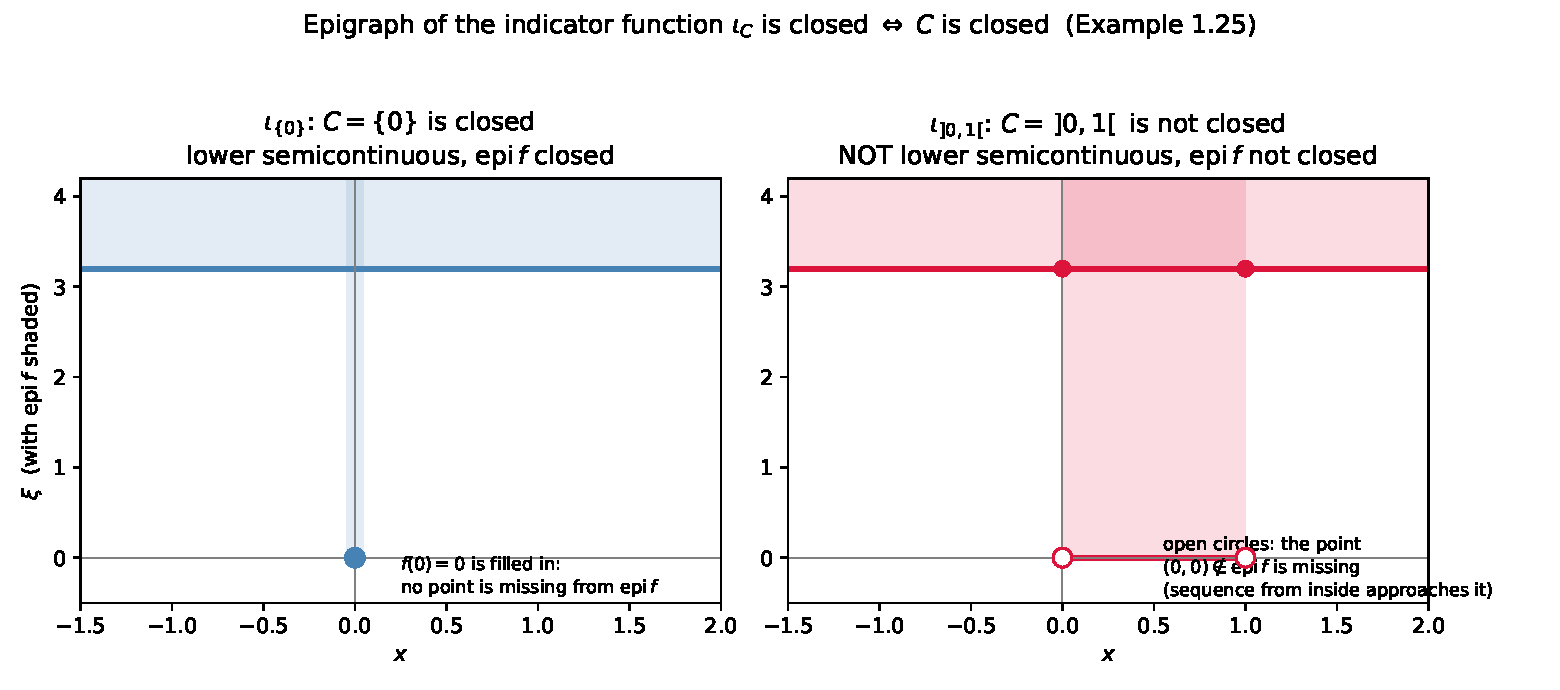
\includegraphics[width=0.92\linewidth]{fig_lsc_epigraph.pdf}
  \end{center}
  \small \textbf{Left:} $\iota_{\{0\}}$ (value $0$ at $x=0$, $+\infty$
  elsewhere): $\{0\}$ is closed, so $\iota_{\{0\}}$ is lsc and its epigraph
  (shaded) is a closed set -- the dip at $x=0$ is filled in, no boundary
  point is missing. \textbf{Right:} $\iota_{\,]0,1[}$ (value $0$ on
  $\,]0,1[\,$, $+\infty$ elsewhere): $\,]0,1[\,$ is not closed, so
  $\iota_{\,]0,1[}$ is \emph{not} lsc; the open circles mark the points
  $(0,0)$ and $(1,0)$ that a sequence from inside the shaded epigraph
  approaches but that are \emph{not} themselves in the epigraph. This
  instantiates Example~1.25, coming up shortly.
\end{frame}

\begin{frame}{1.10 Example 1.22: A Continuous Extended-Real-Valued Function}
  \begin{block}{Example 1.22}
    Set
    \[
      f:\R\to[-\infty,+\infty]: x\mapsto
      \begin{cases}
        1/x, & x>0;\\
        +\infty, & \text{otherwise.}
      \end{cases}
    \]
    Then $f$ is continuous on $\R$ (in particular, lsc), and $\cont
    f=\R_{++}$ is a proper open subset of $\R$: continuity does not require
    finiteness everywhere, only that the value ``matches the limit''
    everywhere, including at points where both sides equal $+\infty$.
  \end{block}
  \begin{alertblock}{Key Remark}
    $\cont f\subset\intr\dom f$ always: $f$ cannot be both continuous and
    real-valued on the boundary of its domain (if it were, points just
    outside $\dom f$, where $f=+\infty$, would need to have nearby values
    close to a finite number -- a contradiction). Also note that a
    continuous function \emph{may} take the values $\pm\infty$, as this
    example shows.
  \end{alertblock}
\end{frame}

\begin{frame}{1.10 Lemma 1.23: $\varlimsup$ of $f$ as $y\to x$ via Nets}
  \begin{block}{Formula (1.36) and Lemma 1.23}
    For $\X$ Hausdorff, $f:\X\to[-\infty,+\infty]$, $x\in\X$:
    \[
      \varlimsup_{y\to x} f(y) = \sup_{V\in\mathcal V(x)}\;\inf f(V).
    \]
    Wait -- more precisely the book's quantity is $\varliminf_{y\to x}f(y)$;
    letting $\mathrm N(x)$ denote the set of \emph{all} nets in $\X$
    converging to $x$,
    \[
      \varliminf_{y\to x} f(y) = \min_{(x_a)_{a\in A}\in\mathrm N(x)}\;
      \varliminf f(x_a).
    \]
  \end{block}
  \begin{exampleblock}{Why This Formula Is the Right One}
    The right side is a genuine \emph{minimum} (not just an infimum): among
    \emph{all} nets converging to $x$, the worst-case (smallest) liminf of
    $f$ along the net is achieved by some particular net -- namely, the net
    built from pairs $(y,V)$ with $y\in V\in\mathcal V(x)$, ordered by
    reverse inclusion of $V$, exactly as in the proof of Lemma~1.10. This
    identity is the bridge between the ``net'' definition of lsc (Definition
    1.21) and the more classical ``$\varliminf_{y\to x}$'' notation.
  \end{exampleblock}
\end{frame}

\begin{frame}[allowframebreaks]{1.10 Lemma 1.24: Three Equivalent Faces of Lower Semicontinuity}

  \begin{block}{Lemma 1.24 (central result of this section)}
    Let $\X$ be Hausdorff and $f:\X\to[-\infty,+\infty]$. The following are
    equivalent:
    \begin{enumerate}
      \item[(i)] $f$ is lower semicontinuous.
      \item[(ii)] $\epi f$ is closed in $\X\times\R$.
      \item[(iii)] For every $\xi\in\R$, $\lev_{\le\xi}f$ is closed in $\X$.
    \end{enumerate}
  \end{block}

  \begin{exampleblock}{Proof (i) $\Rightarrow$ (ii)}
    Let $(x_a,\xi_a)_{a\in A}$ be a net in $\epi f$ converging to
    $(x,\xi)$ in $\X\times\R$. Then $f(x)\le\varliminf f(x_a)\le
    \varliminf\xi_a=\xi$ (using lsc, then $f(x_a)\le\xi_a$ from
    $(x_a,\xi_a)\in\epi f$). Hence $(x,\xi)\in\epi f$, so $\epi f$ contains
    all its net limits, i.e., is closed (by the Lemma~1.10 characterization
    of closed sets via nets).
  \end{exampleblock}

  \framebreak

  \begin{exampleblock}{Proof (ii) $\Rightarrow$ (iii)}
    Fix $\xi\in\R$ and let $(x_a)_{a\in A}$ be a net in $\lev_{\le\xi}f$
    converging to $x$. Then $(x_a,\xi)_{a\in A}$ is a net in $\epi f$
    converging to $(x,\xi)$. Since $\epi f$ is closed, $(x,\xi)\in\epi f$,
    i.e., $x\in\lev_{\le\xi}f$. So $\lev_{\le\xi}f$ contains all its net
    limits: it is closed.
  \end{exampleblock}

  \begin{exampleblock}{Proof (iii) $\Rightarrow$ (i)}
    Fix $x\in\X$, let $x_a\to x$, and set $\mu=\varliminf f(x_a)$. It
    suffices to show $f(x)\le\mu$; assume $\mu<+\infty$ (else trivial).
    \textbf{Step 1.} By Fact~1.15(ii), some subnet $(x_{k(b)})_{b\in B}$
    has $f(x_{k(b)})\to\mu$. \textbf{Step 2.} Fix
    $\xi\in\,]\mu,+\infty[\,$: eventually $f(x_{k(b)})\le\xi$, so
    eventually $x_{k(b)}\in\lev_{\le\xi}f$. \textbf{Step 3.} Since
    $x_{k(b)}\to x$ (Fact~1.9) and $\lev_{\le\xi}f$ is closed, $x\in
    \lev_{\le\xi}f$, i.e., $f(x)\le\xi$. \textbf{Step 4.} Letting
    $\xi\downarrow\mu$ gives $f(x)\le\mu$, as required.
  \end{exampleblock}

\end{frame}

\begin{frame}{1.10 Example 1.25: Indicator Functions (Our Second Running Example)}
  \begin{block}{Example 1.25: The Indicator Function}
    Let $\X$ be Hausdorff, $C\subset\X$. The \textbf{indicator function} of
    $C$ is
    \[
      \iota_C:\X\to[-\infty,+\infty]: x\mapsto
      \begin{cases}
        0, & x\in C;\\
        +\infty, & \text{otherwise.}
      \end{cases}
    \]
    $\iota_C$ is lower semicontinuous \textbf{if and only if} $C$ is closed.
  \end{block}
  \begin{exampleblock}{Proof, and the Concrete Instance $\X=\R$}
    \textbf{Step 1.} $\lev_{\le\xi}\iota_C=\varnothing$ if $\xi<0$, and
    $\lev_{\le\xi}\iota_C=C$ if $\xi\ge0$. \textbf{Step 2.} By Lemma~1.24,
    $\iota_C$ is lsc iff every $\lev_{\le\xi}\iota_C$ is closed, i.e., iff
    $C$ (and $\varnothing$) is closed.

    \smallskip
    \textbf{Concretely (matching the figure two slides back):} take
    $C=\{0\}$ (closed in $\R$) $\Rightarrow$ $\iota_{\{0\}}$ is lsc, epigraph
    closed. Take $C=\,]0,1[\,$ (not closed in $\R$) $\Rightarrow$
    $\iota_{\,]0,1[}$ is \emph{not} lsc: e.g., the sequence $x_n=1/n\to0$
    lies in $\,]0,1[\,$ with $\iota_{\,]0,1[}(x_n)=0$ for all $n$, so
    $\varliminf \iota_{\,]0,1[}(x_n)=0 < \iota_{\,]0,1[}(0)=+\infty$,
    violating Definition~1.21.
  \end{exampleblock}
\end{frame}

\begin{frame}{1.10 Preserving Lower Semicontinuity: Sup, Min, Sums, Composition}
  \begin{block}{Lemma 1.26 and Lemma 1.27}
    Let $(f_i)_{i\in I}$ be lsc functions from $\X$ to $[-\infty,+\infty]$.
    Then $\sup_{i\in I}f_i$ is lsc (immediate from Lemma~1.6(i): an
    intersection of closed epigraphs is closed); if $I$ is finite,
    $\min_{i\in I}f_i$ is lsc too (from Lemma~1.6(ii): a \emph{finite} union
    of closed sets is closed). If $(f_i)_{i\in I}$ is a \emph{finite} family
    of lsc functions to $\,]-\infty,+\infty]$ and $(\alpha_i)_{i\in I}$ are
    in $\R_{++}$, then $\sum_{i\in I}\alpha_i f_i$ is lsc.
  \end{block}
  \begin{exampleblock}{Proof Sketch of the Sum Rule (two lsc functions)}
    For $f,g$ lsc and $x_a\to x$: by Lemma~1.16 (superadditivity of
    $\varliminf$),
    \[
      (f+g)(x) = f(x)+g(x) \;\le\; \varliminf f(x_a)+\varliminf g(x_a)
      \;\le\; \varliminf\big(f(x_a)+g(x_a)\big) = \varliminf(f+g)(x_a).
    \]
    The general finite case follows by induction on $|I|$.
  \end{exampleblock}
  \begin{block}{Lemma 1.28: Composition with a Continuous Map}
    If $T:\X\to\Y$ is continuous and $g:\Y\to[-\infty,+\infty]$ is lsc, then
    $f=g\circ T$ is lsc: continuity ``transports'' convergent nets, and lsc
    ``transports'' the liminf inequality, so the two compose seamlessly.
  \end{block}
\end{frame}

\begin{frame}[allowframebreaks]{1.10 Theorem 1.29 (Weierstrass): Existence of Minimizers}

  \textbf{Intuition.} The classical Weierstrass theorem says a continuous
  function on a compact set attains its minimum. Lower semicontinuity is the
  exact weakening of continuity needed to keep this conclusion true --
  upward jumps cannot hide a lower value that the infimum is trying to
  reach.

  \begin{block}{Theorem 1.29 (Weierstrass)}
    Let $\X$ be Hausdorff, $f:\X\to[-\infty,+\infty]$ lsc, and $C\subset\X$
    compact with $C\cap\dom f\ne\varnothing$. Then $f$ \textbf{achieves its
    infimum over $C$}, i.e., $\min f(C)$ exists.
  \end{block}

  \begin{exampleblock}{Proof, Step by Step}
    \textbf{Step 1.} By definition of $\inf f(C)$, there is a minimizing
    sequence $(x_n)_{n\in\N}$ of $f+\iota_C$ (i.e., $x_n\in C$ and
    $f(x_n)\to\inf f(C)$).

    \smallskip
    \textbf{Step 2.} By compactness of $C$ (Fact~1.11) there is a subnet
    $(x_{k(b)})_{b\in B}$ converging to some $x\in C$.

    \smallskip
    \textbf{Step 3.} Since $(f(x_n))_{n\in\N}$ converges to $\inf f(C)$,
    every subnet of it converges to the same value, so $f(x_{k(b)})\to
    \inf f(C)\le f(x)$ -- wait, we instead use lower semicontinuity
    directly: $f(x)\le\varliminf f(x_{k(b)}) = \lim f(x_{k(b)}) = \inf
    f(C)$.

    \smallskip
    \textbf{Conclusion.} Combined with $f(x)\ge\inf f(C)$ (since $x\in C$),
    we get $f(x)=\inf f(C)$: the infimum is achieved at $x$, i.e.,
    $\min f(C)=f(x)$.
  \end{exampleblock}

  \begin{alertblock}{Why This Theorem Is Fundamental}
    Theorem~1.29 is the single most-used existence tool in convex
    optimization (Chapters 11+): to prove a minimizer exists, one shows the
    objective is lsc and that minimization can be restricted to a compact
    set (e.g., a sublevel set that happens to be compact).
  \end{alertblock}

\end{frame}

\begin{frame}{1.10 Marginal Functions and the Lower Semicontinuous Envelope}
  \begin{block}{Lemma 1.30: Marginal Functions Preserve Lower Semicontinuity}
    Let $\Y$ be a compact Hausdorff space and $\varphi:\X\times\Y\to
    [-\infty,+\infty]$ lsc. Then the \textbf{marginal function}
    $f:\X\to[-\infty,+\infty]: x\mapsto\inf\varphi(x,\Y)$ is lsc, and
    $f(x)=\min\varphi(x,\Y)$ for every $x$ (minimizing out a compact
    variable preserves lsc and always attains its infimum, by
    Theorem~1.29 applied to $\{x\}\times\Y$).
  \end{block}
  \begin{block}{Definition 1.31: Lower Semicontinuous Envelope}
    For any $f:\X\to[-\infty,+\infty]$, the \textbf{lsc envelope} is
    \[
      \bar f = \sup\{g:\X\to[-\infty,+\infty] \mid g\le f,\; g \text{ lsc}\}.
    \]
    I.e., $\bar f$ is the \emph{largest} lsc minorant of $f$ -- the best
    ``lsc approximation from below.''
  \end{block}
  \begin{block}{Lemma 1.32 (Key Facts About $\bar f$)}
    $\bar f$ is the largest lsc function majorized by $f$; $\epi\bar f$ is
    closed; $\dom f\subset\dom\bar f\subset\overline{\dom f}$;
    $\bar f(x)=\varliminf_{y\to x}f(y)$ for every $x$; $f$ is lsc at $x$ iff
    $\bar f(x)=f(x)$; and $\epi\bar f=\overline{\epi f}$ (the epigraph of
    the envelope is exactly the closure of the original epigraph).
  \end{block}
\end{frame}

%% ══════════════════════════════════════════════════════════════════════════
\section{1.11 Sequential Topological Notions}
%% ══════════════════════════════════════════════════════════════════════════

\begin{frame}{1.11 Sequentially Closed, Sequentially Compact}
  \textbf{Intuition.} Since sequences are indexed by $\N$ only, they may
  fail to detect everything that nets can detect in a general topological
  space. This section defines the ``sequential'' versions of our topological
  notions and records exactly when they coincide with the originals.

  \begin{block}{Sequentially Closed, Sequentially Compact}
    $C\subset\X$ (Hausdorff) is \textbf{sequentially closed} if the limit of
    every convergent \emph{sequence} in $C$ lies in $C$. Every closed set is
    sequentially closed, but \emph{not conversely} in general (a
    counterexample appears later in the book, Example 3.33). $C$ is
    \textbf{sequentially compact} if every sequence in $C$ has a
    \emph{subsequence} converging to a point of $C$.
  \end{block}

  \begin{block}{Sequential Continuity and Sequential (Semi-)Continuity}
    Replacing nets by sequences (and subnets by subsequences) throughout
    Fact~1.19 and Definition~1.21 gives \textbf{sequential continuity} and
    \textbf{sequential lower/upper semicontinuity}.
  \end{block}
\end{frame}

\begin{frame}{1.11 Sequential Analogues of Lemmas 1.12, 1.14, 1.24}
  \begin{block}{Lemma 1.34, Lemma 1.35}
    If $C$ is sequentially compact, then $C$ is sequentially closed, and
    every sequentially closed subset of $C$ is sequentially compact
    (Lemma~1.34). If, moreover, $(x_n)_{n\in\N}$ in $C$ has a \emph{unique}
    sequential cluster point $x$, then $x_n\to x$ (Lemma~1.35) -- exact
    sequential mirrors of Lemma~1.12 and Lemma~1.14.
  \end{block}
  \begin{block}{Lemma 1.36}
    For $f:\X\to[-\infty,+\infty]$, the following are equivalent: (i) $f$ is
    sequentially lsc; (ii) $\epi f$ is sequentially closed in $\X\times\R$;
    (iii) every $\lev_{\le\xi}f$ ($\xi\in\R$) is sequentially closed in
    $\X$ -- the exact sequential mirror of Lemma~1.24.
  \end{block}
  \begin{alertblock}{Remark 1.37: Sequential Spaces}
    $\X$ is \textbf{sequential} if sequentially closed $=$ closed for every
    subset. In sequential spaces, lsc and sequential lsc coincide (and
    continuity coincides with sequential continuity for every target
    space). \textbf{Caution:} even in Hausdorff sequential spaces, compact
    and sequentially compact can still differ. Every metric space (next
    section) is sequential -- this is why $\R^n$ analysis never needs to
    worry about the net/sequence distinction.
  \end{alertblock}
\end{frame}

%% ══════════════════════════════════════════════════════════════════════════
\section{1.12 Metric Spaces}
%% ══════════════════════════════════════════════════════════════════════════

\begin{frame}{1.12 Metric Spaces: Distance, Balls, Metric Topology}
  \textbf{Intuition.} A metric space is the familiar setting of ``distance
  between two points,'' exactly like $\R^n$ with the Euclidean norm. Every
  metric space is automatically Hausdorff and, crucially, \emph{sequential}
  -- sequences suffice for everything.

  \begin{block}{Distance, Diameter, Distance to a Set}
    Let $(\X,d)$ be a metric space, $C\subset\X$. The \textbf{diameter} is
    $\diam C=\sup_{(x,y)\in C\times C} d(x,y)$. The \textbf{distance to
    $C$} is $d_C:\X\to[0,+\infty]: x\mapsto\inf d(x,C)$ (with
    $d_\varnothing\equiv+\infty$).
  \end{block}
  \begin{block}{Balls and the Metric Topology}
    The \textbf{closed} and \textbf{open balls} of center $x\in\X$, radius
    $\rho\in\R_{++}$ are $B(x;\rho)=\{y\in\X \mid d(x,y)\le\rho\}$ and
    $\{y\in\X \mid d(x,y)<\rho\}$. The \textbf{metric topology} of $\X$ has
    the family of all open balls as a base. $\X$ is \textbf{metrizable} if
    some metric induces its topology. A sequence $x_n\to x$ iff $d(x_n,x)
    \to0$.
  \end{block}
  \begin{alertblock}{Consequence}
    Every metric space is a sequential Hausdorff space: closedness,
    continuity, and lower semicontinuity all coincide with their sequential
    counterparts (Remark~1.37).
  \end{alertblock}
\end{frame}

\begin{frame}{1.12 Facts 1.38--1.39 and Lemmas 1.40--1.41}
  \begin{block}{Fact 1.38, Fact 1.39}
    Let $\X$ be a metric space, $\Y$ Hausdorff, $T:\X\to\Y$: $T$ is
    continuous iff $T$ is sequentially continuous (Fact~1.38). A subset $C$
    of a metric space is compact iff it is sequentially compact
    (Fact~1.39): in metric spaces, the net-based and sequence-based
    definitions of compactness are literally the same property.
  \end{block}
  \begin{block}{Lemma 1.40, Lemma 1.41}
    If $C\cap B(z;n)$ is closed for every strictly positive integer $n$
    (some fixed $z$), then $C$ is closed (Lemma~1.40: a sequence in $C$ is
    bounded, hence trapped in some fixed ball, where closedness already
    applies). A \textbf{compact} subset of a metric space is
    \textbf{closed and bounded} (Lemma~1.41; the converse needs
    finite-dimensionality and is \emph{not} claimed here).
  \end{block}
  \begin{block}{Lemma 1.42}
    For $f:\X\to[-\infty,+\infty]$, $x\in\X$, and $\mathrm S(x)$ the set of
    all sequences converging to $x$: $\varliminf_{y\to x}f(y) =
    \min_{(x_n)\in\mathrm S(x)}\varliminf f(x_n)$ -- the sequential mirror
    of Lemma~1.23, valid because metric spaces are sequential.
  \end{block>
\end{frame}
